\documentclass[applsci,article,accept,moreauthors,pdftex]{Definitions/mdpi} 
\usepackage{subcaption}  % Add this in your preamble
\usepackage[ruled,vlined]{algorithm2e}
\usepackage{tikz}
\usetikzlibrary{shapes.geometric, arrows}
\tikzstyle{startstop} = [rectangle, rounded corners, minimum width=3cm, minimum height=1cm,text centered, draw=black]
\tikzstyle{io} = [trapezium, trapezium left angle=70, trapezium right angle=110, minimum width=0.5cm, minimum height=1cm, text centered, draw=black ]
\tikzstyle{process} = [rectangle, minimum width=3cm, minimum height=1cm, text centered, draw=black]
\tikzstyle{decision} = [diamond, minimum width=3cm, minimum height=2cm, text centered, draw=black]
\tikzstyle{arrow} = [thick,->,>=stealth]

\firstpage{1} 
\makeatletter 
\setcounter{page}{\@firstpage} 
\makeatother
\pubvolume{0}
\issuenum{0}
\articlenumber{0}
\pubyear{202y}
\copyrightyear{2024}
\externaleditor{Academic Editor: Silvio Cocuzza} % For journal Automation, please change Academic Editor to "Communicated by"
\datereceived{dd mm yyyy} 
\dateaccepted{dd mm yyyy} 
\datepublished{} 
\hreflink{https://doi.org/} % If needed use \linebreak


%\usepackage{cite}
%\usepackage{amsmath,amssymb,amsfonts}
%\usepackage{algorithmic}
%\usepackage{graphicx}
%\usepackage{textcomp}

%\usepackage{balance}
%\usepackage{bm}


% The following line should be uncommented if the LaTeX file is uploaded to arXiv.org
%\pdfoutput=1

% Add packages and commands here. The following packages are loaded in our class file: fontenc, inputenc, calc, indentfirst, fancyhdr, graphicx, epstopdf, lastpage, ifthen, lineno, float, amsmath, setspace, enumitem, mathpazo, booktabs, titlesec, etoolbox, tabto, xcolor, soul, multirow, microtype, tikz, totcount, changepage, paracol, attrib, upgreek, cleveref, amsthm, hyphenat, natbib, hyperref, footmisc, url, geometry, newfloat, caption

%% Please use the following mathematics environments: Theorem, Lemma, Corollary, Proposition, Characterization, Property, Problem, Example, ExamplesandDefinitions, Hypothesis, Remark, Definition, Notation, Assumption
%% For proofs, please use the proof environment (the amsthm package is loaded by the MDPI class).

% Full title of the paper (Capitalized)
\Title{Identification of Elephant Rumbles in Seismic Infrasonic Signals Using Spectrogram-based Machine Learning}

% MDPI internal command: Title for citation in the left column
\TitleCitation{Identification of Elephant Rumbles in Seismic Infrasonic Signals Using Spectrogram-based Machine Learning}

% Author Orchid ID: enter ID or remove command
\newcommand{\orcidauthorA}{0000-0002-8619-1156} % Add \orcidA{} behind the author's name
\newcommand{\orcidauthorB}{0000-0003-3445-4767} % Add \orcidB{} behind the author's name

% Authors, for the paper (add full first names)
\Author{A.~M.~J.~V.~Costa, C.~S.~Pallikkonda, H.~H.~R.~Hiroshan, G.~R.~U.~Y.~Gamlath, C.~U.~S.~Edussooriya, and S.~R.~Munasinghe \orcidA{0000-0003-3445-4767}}
%MDPI: Please carefully check the accuracy of names and affiliations. 
%MDPI: Please confirm whether it is number 2


% MDPI internal command: Authors, for metadata in PDF
\AuthorNames{}

% MDPI internal command: Authors, for citation in the left column
\AuthorCitation{Costa A. M. J. V.; Pallikonda C. S.; Hiroshana H. H. R.; Gamlath G. R. U. Y.; Edussooriya C. U. S.; Munasinghe S.R.}
% If this is a Chicago style journal: Lastname, Firstname, Firstname Lastname, and Firstname Lastname.

% Affiliations / Addresses (Add [1] after \address if there is only one affiliation.)
\address{Department of Electronic and Telecommunication Engineering, University of Moratuwa, Moratuwa 10400, Sri Lanka\\
Dept. of Global Development, CALS, Cornell University, NY 14853, USA}

% Contact information of the corresponding author
\corres{Correspondence: \hl {srm278@cornell.edu}}
%MDPI: Newly added, please confirm.
%MDPI: E-mails are different from redmine, please confirm.

% Current address and/or shared authorship

%%\firstnote{Current address: Affiliation 3} 
%%\secondnote{These authors contributed equally to this work.}
%//////////////
% The commands \thirdnote{} till \eighthnote{} are available for further notes

%\simplesumm{} % Simple summary

%\conference{} % An extended version of a conference paper

% Abstract (Do not insert blank lines, i.e. \\) 
\abstract{This paper presents several machine-learning methods and highlights the most effective one for detecting elephant rumbles in infrasonic seismic signals. The design and implementation of electronic circuitry to amplify, filter, and digitize the seismic signals captured through geophones are presented. The process converts seismic rumbles to the spectrogram and the existing methods of spectrogram feature extraction and appropriate machine learning algorithms are compared on their merit of automatic seismic rumble identification. A novel method of denoising the spectrum that leads to enhanced accuracy in identifying seismic rumbles is presented. It was experimentally found that the combination of the Mel frequency cepstral coefficient (MFCC) feature extraction method and the Ridge classifier machine learning algorithm gives the highest accuracy of 97\% in detecting infrasonic elephant rumbles hidden in seismic signals. The trained machine learning algorithm can run quite efficiently on general-purpose embedded hardware such as Raspberry Pi, hence the method provides a cost-effective and scalable platform to develop a tool to remotely localize elephants, which would help mitigate the human-elephant conflict.}

\keyword{Infrasonic elephant rumbles; spectrogram; Mel-frequency cepstral coefficients; Hjorth parameters; Geophone; seismic waves.} 

\begin{document}
%\setcounter{section}{-1} %% Remove this when starting to work on the template.
\section{Introduction}
Elephants use different vocalization patterns to communicate between herds and each other for food, water, mating, and warning. Among these patterns, the infrasonic rumbles have a very specific significance in long-range communication \cite{nair2009vocalizations}. Elephant rumbles have acoustic and seismic components. The acoustic component propagates through the air as a three-dimensional wave, and gets attenuated through the foliage fairly quickly. The seismic component on the other hand propagates through the ground as a two-dimensional Rayleigh wave and therefore, travels a longer distance compared to the acoustic component. Elephant's foot is believed to have the capability of a seismic transponder to facilitate long-range seismic infrasonic communication. These seismic signals can be a powerful component of an elephant’s communication system, serving crucial functions such as mate finding, prey detection, and interspecific and intraspecific warnings \cite{o2000seismic}. The attenuation of seismic waves during transmission increases monotonically with frequency, hence the range of 10 Hz to 40 Hz is considered the "sweet zone" for seismic signal propagation. Elephant rumbles, which have a fundamental frequency of around 20 Hz \cite{payne1986infrasonic}, fall within this sweet zone, allowing them to communicate through the ground. The elephant rumbles that propagate as Rayleigh waves through the ground can be captured using geophones \cite{gunther2004seismic}.\par
Detecting and localizing wild elephants through airborne rumbles encounter certain challenges that impede its effectiveness. Airborne signals, though easy to detect, attenuate rapidly limiting the range over which elephants can be identified. The amplitude of a Rayleigh wave during ground surface transmission is inversely proportional to
the square root of the distance, with a loss of 3 dB for every doubling of the distance. In airborne signals,
amplitude is inversely proportional to the distance, with a loss of 6 dB for every doubling of the distance. Factors such as weather, time of day, scattering, and reflections due to objects, and trees also attenuate the airborne signal \cite{o2000seismic}. The seismic wave undergoes a lower attenuation compared to the airborne wave, hence the detectable range of the seismic component of a rumble is greater than that of the airborne acoustic component \cite{sayakkara2017eloc}. In \cite{wijayakulasooriya}, a method is proposed to detect elephant rumbles using the shape of the formant frequency tracks of a rumble. However, the assumption in this research that the first two formant frequencies remain stationary is controversial \cite{zeppelzauer2015towards}. In \cite{Hao}, a template matching method is used for rumble identification in which a reference feature template is used to clarify whether or not a test sample contains a rumble. This method delivers subpar performance with a 78.6\% detection rate in which 78.2\% is false positives as reported in \cite{zeppelzauer2015}. In \cite{zeppelzauer2015}, seismic elephant rumbles are identified using support vector machines (SVMs) and signal enhancement, which has achieved an 88.2\% detection rate with 13.7\% false positives. In  \cite{Reinwald2021}, elephant localization using an array of infrasonic seismic rumble detectors is demonstrated. Among the limited research conducted in detecting seismic elephant rumbles signal acquisition and signal processing have not yet been fully investigated. There is a clear research gap and a need to develop the right signal acquisition and processing methods to improve seismic elephant rumble detection.

This research intends to explore this gap and propose the most effective signal acquisition and signal processing methods for infrasonic seismic elephant rumble detection. After experimentally evaluating various feature extraction techniques, we observe that the three machine learning (ML) algorithms: Ridge Classifier, Decision Tree Classifier, and Light Gradient Boosting Machine (LGBM) classifier provide the best results when Mel frequency cepstral coefficients (MFCC), Hjorth parameters, and spectral energy distributions, respectively, are used as features in identifying infrasonic seismic elephant rumbles. We further find that the Ridge classifier and MFCC feature extraction method together achieves the highest accuracy of 97\%, which is the best performance in elephant rumble detection to date. This outcome will help devise a tool to detect wild elephants at a distance and timely alert the villagers in the neighborhood to mitigate the human-elephant conflict \cite{prakash}.

\section{Spectrogram of Infrasonic Seismic Signals}
\subsection{Overview of Signal Acquisition and Processing}
The seismic elephant rumbles are in the micro-volt range. They are picked up by geophones, and amplified electronically to a level suitable for signal processing. The amplified seismic signal is then bandpass filtered to within the 5Hz to 150Hz range, which is the typical bandwidth of elephant infrasonic rumble. This filtering ensures that noise and other unwanted signals are removed, enhancing the signal quality. To achieve the desired voltage gain, the signal is guided through a variable gain amplifier in which the gain is optimally adjusted. Then, the signal is sent to an analog-to-digital converter (ADC) for digitization. As an additional precaution, a voltage clipping stage is employed to safeguard against any potential voltage spikes that could adversely impact the data integrity. The digital signal is transmitted to a Raspberry Pi single-board computer through the I2C communication protocol. In the Raspberry Pi, the spectrogram features are extracted and fed to a trained machine-learned algorithm to determine if the spectrogram contains an elephant rumble. The overview of the system is shown in Figure~\ref{fig:dh-prodecrrnn}.
\begin{figure*}
	\centering
	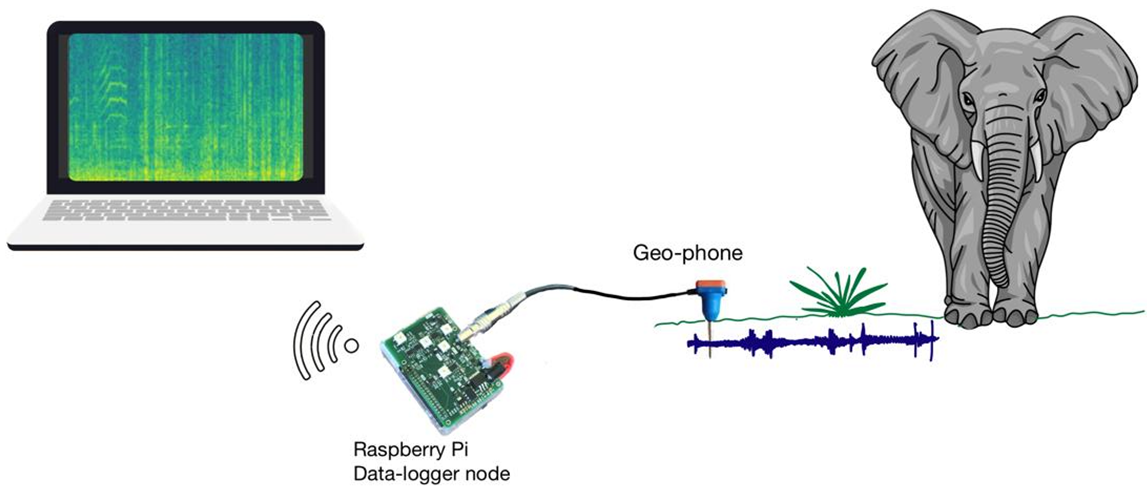
\includegraphics[width=0.9\columnwidth]{figures/overview.png} 
	\caption{An overview of the system. The system captures infrasonic seismic signals using geophones. The captured signals are conditioned and transmitted to a computer for signal processing and implement machine learning algorithm to detect elephant rumbles.} \label{fig:dh-prodecrrnn}
\end{figure*}

\subsection{Electronic Circuitry}
Figure \ref{hw design} shows the seismic signal acquisition workflow which involves the geophone, amplifier I, bandpass filter, amplifier II, clamping and clipping circuitry, and the 16-bit ADC.  
\begin{figure}[h]
	\begin{center}
		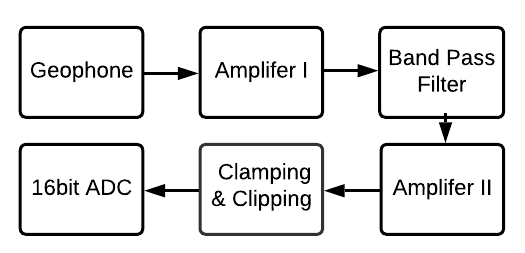
\includegraphics[width=2.5in]{figures/cct_block}\\
		\includegraphics[width=2.5in]{figures/circuit}
		\caption{Seismic signal processing workflow (above), and the electronic circuit (below).}
		\label{hw design}
	\end{center}
\end{figure}

\subsubsection{The Geophone}
The geophone consists of a coil of wire suspended between magnets with a mass attached to it. When seismic waves pass through the ground, the mass vibrates, generating electrical signals proportional to the vertical component of the ground vibration. This research uses SG-05 geophone of which the technical specifications are listed in Table \ref{table:geophone}. 
\begin{table}[h]
	\caption{Geophone SG-05 Technical Specifications}
	\centering
	\begin{tabular}{l r}
		\hline\hline
		Property & Value\\
		\hline
		Natural frequency &  5 Hz\\
		Sensitivity &  80 V/ms$^{-1}$\\
		Spurious frequency &  150 Hz\\
		Weight  &  22.7 g\\
		Operating temprature  &  -40$^{\circ}$C to +80$^{\circ}$C\\
		\hline
	\end{tabular}
	\label{table:geophone}
\end{table}
\subsubsection{Amplifier I}
The micro-volt signal generated by the geophone is amplified by Amplifier I, which is an instrumental amplifier. It accepts a differential input and eliminates the common mode noise significantly with a high common mode rejection ratio (CMRR). Being an integrated circuit, it has a lower instrumental noise and offset. The passive components of the circuit were carefully selected considering the tolerances, as they can affect the signal quality significantly. The amplifier has a gain of 500 in this stage.

\subsubsection{Band Pass Filter and Anti-Aliasing}
The seismic elephant rumble spread over infrasonic frequencies, hence other frequencies the geophone picks up are to be removed. For this, a third-order Butterworth filter is used. Since the Butterworth filter has a flat passband gain, the filtering will uniformly affect the amplitudes of the passband frequencies in the geophone signal. This filter further acts as an anti-aliasing filter before the ADC. The filter implementation employs a Sallen-key topology and uses a low-noise operational amplifier (OPAmp) \cite{zumbahlen2007phase}. Figure \ref{fig:bandpass1} shows the gain and phase response of the filter.
\begin{figure}[h]
	\centering   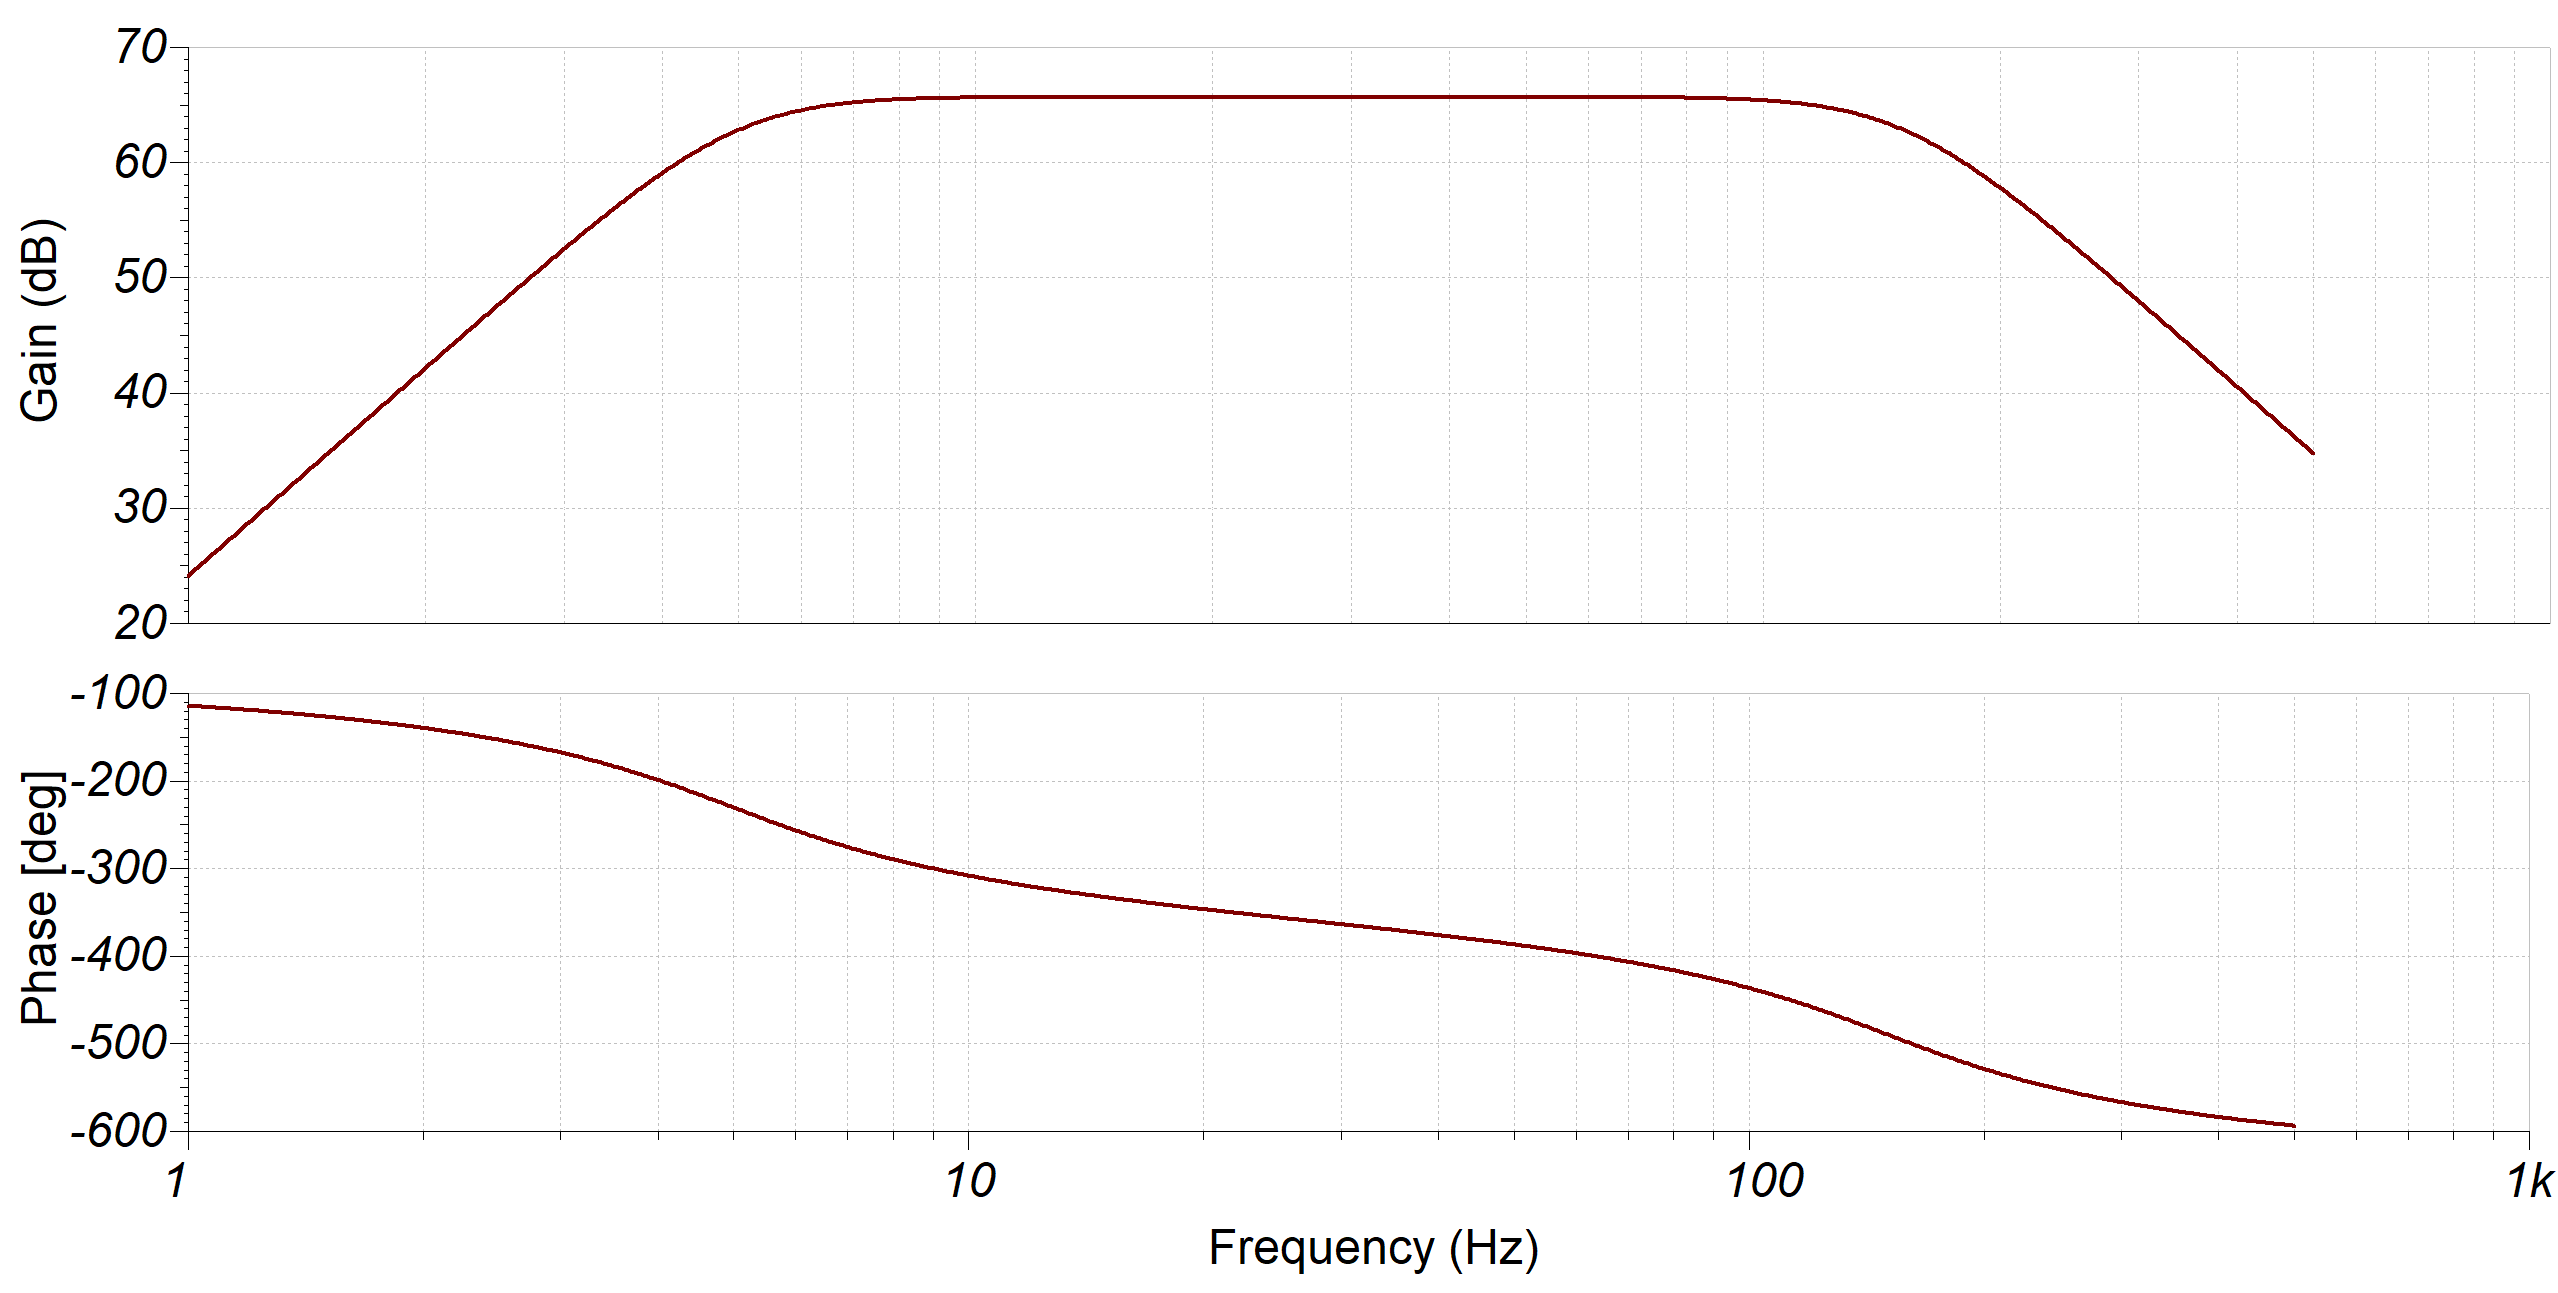
\includegraphics[width=1\columnwidth]{figures/BodePlot}
	\caption{Frequency response of the Bandpass filter: magnitude(above) and phase(below) responses}
	\label{fig:bandpass1}
\end{figure}
\subsubsection{Amplifier II}
After the band-pass filtering, the signal is mostly infrasonic, and it may or may not contain an elephant rumble. The signal is still weak and therefore it is amplified again using the Amplifier II, which is an inverting amplifier with a variable gain that is adjusted using a variable resistor shown in Figure~\ref{hw design} (below). Amplifier II elevates the signal to the full voltage range of 0 V–3.3 V. The total amplification therefore is in the range of 3000-6000.
\subsubsection{Clamping and Clipping Circuit}
The voltage clipping circuit limits the analog signal to a safe range of 0 V to 3.3 V before feeding it into the ADC. This protective measure serves two primary purposes: limiting the analog signal range; and protecting against voltage spikes. The voltage clamp circuit adds a DC offset to the signal to make it a positive voltage before feeding it to the ADC.

\subsubsection{Analog to Digital Converter}
The 16-bit ADC converts the amplified band-limited analog signal to digital format. Considering the geophone signal bandwidth of 150 Hz, the sampling rate is selected as 475 samples per second so that aliasing does not happen. One elephant rumble acquired is illustrated in Figure. \ref{fig_rumblefiltered}.
\begin{figure*}[t]
	\centering   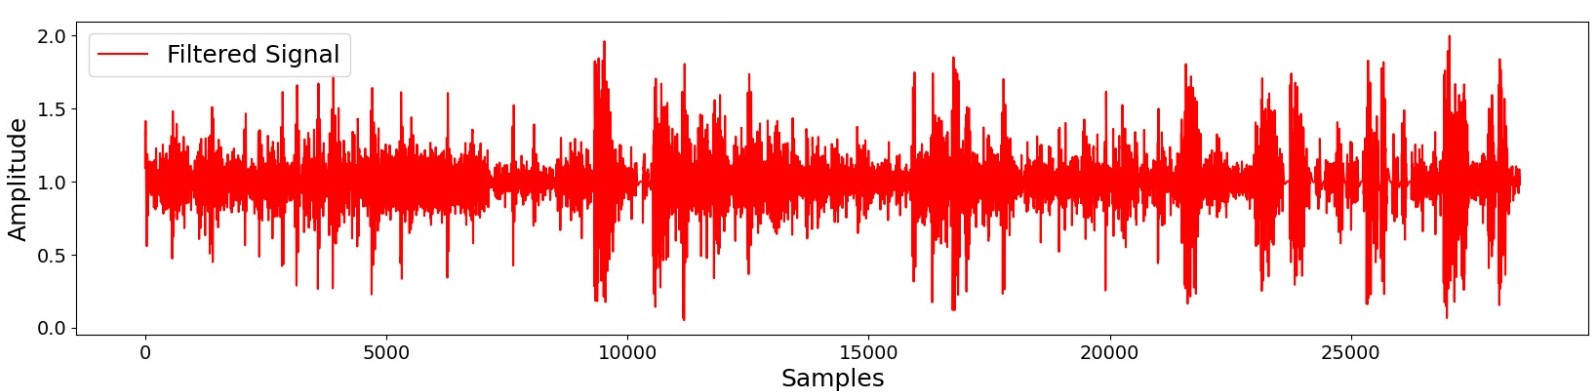
\includegraphics[width=1\columnwidth]{figures/rumblefiltered}
	\caption{An elephant rumble after filtering}
	\label{fig_rumblefiltered}
\end{figure*}
The signal spectrum of the rumble after filtering is shown in Fig.\ref{figure/rumblespecrum}
\begin{figure}[h]
	\centering   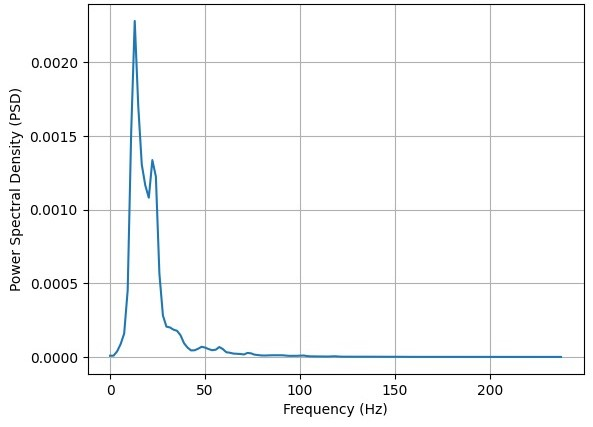
\includegraphics[width=0.7\columnwidth]{figures/rumblespectrum}
	\caption{The spectrum of an elephant rumble}
	\label{fig_rumblespectrum}
\end{figure}
The digitized signal in a 10 Hz-150 Hz band, is then transferred to the Raspberry Pi single-board computer for further processing. 
\subsubsection{Sensitivity}
The sensitivity of the 16-bit ADC with a range of 3.3 V can be obtained as
\begin{equation}
	S_{ADC}=\frac{3.3 \text{ V}}{2^{16} - 1} = 50.354\ \mu \text{V}.\label{eq:Sadc}
\end{equation}
Given the geophone sensitivity $S_{G}$ and the amplification factor $g$, the sensitivity  of the system $S_{s}$ is given by 
\begin{equation}
	S_{s} = \frac{S_{ADC}}{gS_{G}}.
	\label{eq:sens}
\end{equation}
The sensitivity of the geophone is $S_{G}=80 \text{ V/ms}^{-1}$ (see Table \ref{table:geophone}), and with $g$=3000, $S_{s}=0.3147$ ms$^{-1}$. 
\subsection {Signal Processing}
\subsubsection{Wavelet Decomposition and Reconstruction}
The wavelet transform is used for the time-frequency decomposition of the seismic signal while also denoising the signal \cite{donoho1995noising}. The wavelet transform decomposes the signal into a sum of wavelets with varying positions and scales, enabling to capture of low-frequency and high-frequency details. Here we employ Daubechies 3 wavelet for the wavelet decomposition and denoising.
\subsubsection{Identification of Frequency Ridges}
A ridge filter is first applied to identify the ridge structures of the spectrogram. Then, the filtered spectrogram is applied to the original spectrogram as a weighting function to enhance it further. At each spatial position $(t, f)$ in the spectrogram $S(t, f)$, where $t$ represents time and $f$ denotes frequency, the partial derivatives (gradients) of the spectrogram were calculated concerning both time and frequency. Then, the gradients are subjected to a Gaussian smoothing process. The structure tensor, which captures the local intensity distribution structure in the spectrogram's neighborhood is then constructed from the smoothed gradients as follows~\cite{zeppelzauer2015towards}:
\begin{align}
	T(t, f) =
	\begin{bmatrix}
		\nabla_t^2 & \nabla_t \cdot \nabla_f  \\
		\nabla_t \cdot \nabla_f  & \nabla_f^2
	\end{bmatrix},
\end{align}
where $T(t, f)$ is the structure tensor at $(t,f)$, $\nabla_t$  is the partial derivative with respect to time, and $\nabla_f$ is the partial derivate with respect to frequency. From the structure tensor, we derive the eigenvalues $\lambda_1$ and $\lambda_2$ using the following expression
\begin{eqnarray}
	\lambda_{1,2}=\frac{1}{2}\left[\nabla_t^2 +\nabla_f^2 \pm \sqrt{(\nabla_t^2-\nabla_f^2)^2 + 4(\nabla_t \cdot \nabla_f)^2}\right].
\end{eqnarray}
When there is an edge-like structure such as a frequency contour in the local neighborhood of the spectrogram, the condition $\lambda_1$  $ >\lambda_2$ is fulfilled. In the case of a perfect edge, $\lambda_2$ becomes zero while the condition $\lambda_1$  $ >\lambda_2$  is still fulfilled. If  $\lambda_1$  $ =\lambda_2$, it indicates that the underlying structure is rotationally symmetric, such as an isolated spectral peak. If both eigenvalues become zero, it suggests that the underlying structure is homogeneous throughout the local neighborhood.
From the eigenvalues of the structure tensor at a given position $(t,f)$ in the spectrogram, the coherence is computed as follows:
\begin{equation}
	c = \frac{\lambda_1-\lambda_2}{\lambda_1+\lambda_2}.
\end{equation}
\subsubsection{Spectrogram Enhancement}\label{subsub-SE}
To enhance the visibility of frequency contours while simultaneously reducing noise, the coherence is used as a weighting function. The enhanced spectrogram, $\hat{S}(t, f)$, is computed as shown in {\bf Algorithm 1}.
\begin{equation}
	\hat{S}(t, f) = S(t, f) \cdot (c(t, f) + 1).
\end{equation}

\begin{algorithm}[tb]
	\SetAlgoNlRelativeSize{-1}
	\caption{Enhanced Spectrogram Calculation}
	\KwData{\textit{s} - Input spectrogram\;}
	\KwResult{Enhanced spectrogram\;}
	Apply ridge filtering (\textit{Ridge\_s}) for \textit{s}\;
	Calculate time gradient (\textit{time\_gradient}) along axis 0\;
	Calculate frequency gradient (\textit{frequency\_gradient}) along axis 1\;
	Calculate tensor elements:
	\begin{align*}
		\textit{tensor\_xx} &= \textit{time\_gradient}^2 \\
		\textit{tensor\_yy} &= \textit{frequency\_gradient}^2 \\
		\textit{tensor\_xy} &= \textit{time\_gradient*frequency\_gradient} \\
	\end{align*}
	Apply Gaussian filtering to \textit{tensor\_xx}, \textit{tensor\_yy}, and \textit{tensor\_xy} to obtain smoothed versions\;
	Calculate eigenvalues $\lambda_1$ and $\lambda_2$ \; 
	Calculate coherence ($\textit{c}$) as:
	\[\textit{c} = \frac{\lambda_1 - \lambda_2}{\lambda_1 + \lambda_2}\]
	Calculate enhanced spectrogram ($\textit{enhanced\_spectrogram}$) as:
	\[\textit{enhanced\_spectrogram} = (10 \cdot \log_{10}(\textit{Ridge\_s})) \cdot (1 + \textit{c})\]
	\Return{\textit{enhanced\_spectrogram}}\;
\end{algorithm}

\begin{algorithm}[tb]
	\SetAlgoNlRelativeSize{-1}
	\caption{Threshold-Based Spectrogram Enhancement}
	\KwData{%
		\textit{s1} - Input spectrogram\;
		
	}
	\KwResult{%
		\textit{final\_spectrogram} - Further Enhanced spectrogram\;
	}
	
	Calculate Threshold values from \textit{s1} - \textit{threshold1, threshold2, threshold3} \;
	\For{$i$ in range($\textit{s1.shape[0]}$)}{
		\For{$j$ in range($\textit{s1.shape[1]}$)}{
			\If{$\textit{s1}[i, j] > \textit{threshold3}$}{
				$\textit{final\_spectrogram}[i, j] = \textit{s1}[i, j] + 5$\;
			}\ElseIf{$\textit{s1}[i, j] > \textit{threshold2}$}{
				$\textit{final\_spectrogram}[i, j] = \textit{s1}[i, j] + 2$\;
			}\ElseIf{$\textit{s1}[i, j] > \textit{threshold1}$}{
				$\textit{final\_spectrogram}[i, j] = \textit{s1}[i, j] - 2$\;
			}\Else{
				$\textit{final\_spectrogram}[i, j] = \textit{s1}[i, j] - 5$\;
			}
		}
	}
	\Return{\textit{final\_spectrogram}}\;
\end{algorithm}

Subsequently, as shown in {\bf Algorithm 2} three distinct percentiles ($25^{\text{th}}$, $50^{\text{th}}$, and $75^{\text{th}}$) are computed based on the input spectrogram, and used as threshold values to partition the spectrogram's pixel intensity values into three categories: low, medium, and high.
The algorithm iterates through each pixel within the spectrogram and applies adjustments contingent on the intensity of the pixel. Pixels with values surpassing the $75^{\text{th}}$ percentile undergo enhancement by adding 5, thus accentuating the regions with the highest intensity. Pixels falling within the range of the $50^{\text{th}}$ and $75^{\text{th}}$ percentiles experience a moderate enhancement of 2, ensuring that mid-level features remain discernible. Pixels below the $50^{th}$ percentile have their intensity reduced by subtracting 2, consequently amplifying the contrast between the background and the features of interest. Finally, for pixels with intensities below $25^{th}$ percentile, a reduction of 5 is applied, maintaining a clear distinction between the lowest-intensity areas and other regions of the spectrogram.
Additionally, following the enhancement process, a Gaussian blur operation is applied. This operation serves to further refine the spectrogram, smoothing out noise and improving its overall quality for more precise feature extraction and interpretation.

\subsubsection{Assessment of Spectrogram Enhancement}
To assess the effectiveness of the spectrogram enhancement algorithm, the structural similarity index (SSIM), which is a widely employed metric in image analysis and quality assessment \cite{wang2004image}, is used. It serves as a valuable tool for comparing two images by evaluating their structural similarity, taking into account luminance, contrast, and structure. SSIM quantifies how well the structural elements of an image, such as edges, textures, and patterns, are preserved when compared to a reference image. It produces a value between -1 and 1, where a score of 1 indicates a perfect similarity, meaning the two images are identical, while lower scores signify increasing dissimilarity. The SSIM index is calculated as follows:
\begin{equation}
	\text{SSIM}(x, y) = \frac{{(2\mu_x\mu_y + c_1)(2\sigma_{xy} + c_2)}}{{(\mu_x^2 + \mu_y^2 + c_1)(\sigma_x^2 + \sigma_y^2 + c_2)}},
\end{equation}
where $\mu_x$ is mean of $x$, $\mu_y$ is mean of $y$, $\sigma_x$ is standard deviation of $x$, $\sigma_y$ is standard deviation of $y$, and $\sigma_{xy}$ is covariance between $x$ and $y$. The constance $c_1$ and $c_2$ are defined by $c_i=(Lk_i)^2; i=1,2$, where $L$ is the dynamic range of pixel values, $k_1=0.01$ and $k_2= 0.03$ are default constants.
\section {Spectral Features for Seismic Elephant Rumble Detection}
The three feature sets: MFCC, Hjorth parameters, and spectral energy distribution, that represent the spectral information of seismic data, are tested in order to determine the effectiveness of extracting spectral features of seismic elephant rumbles.
% \begin{itemize}
% 	\item Mel-frequency cepstral coefficients (MFCC)
% 	\item Hjorth parameters
% 	\item Spectral energy distribution
% \end{itemize}
\subsection{Mel-frequency Cepstral Coefficients}
The MFCCs of a signal provide a characteristic representation of the signal \cite{jurafsky}. When extracting MFCCs, the signal is divided into overlapping frames of fixed 25 ms. The frames are shifted by 50\% to create an overlap to ensure continuity. On each frame, a  Hamming window is applied to taper the signal towards the frame boundaries. This is done to enhance the harmonics, smooth the edges, and reduce the edge effect while taking the discrete Fourier transform (DFT)~\cite{oppenheim1999discrete} of the signal. Each windowed frame is converted into a magnitude spectrum by applying DFT as follows:
\begin{equation}
	X(k) = \sum_{n=0}^{N-1} x(n) \cdot e^{-j\frac{2\pi}{N}nk}, \quad k = 0, 1, \ldots, N-1,
\end{equation}
where $X(k)$ is DFT of the input sequence $x(n)$, $N$ is number of samples in the sequence, and $k$ is frequency index.
The Mel spectrum is obtained by applying a Mel-filter bank to the Fourier-transformed signal. The approximation of the Mel frequency scale from the actual frequency is expressed as follows.
\begin{equation}
	m = 2595 \log_{10}\left(1 + \frac{f}{700}\right),
\end{equation}
where $m$ is Mel-frequency scale of the actual frequency $f$ in Hz. The Mel spectrum of the magnitude spectrum $X(k)$ is computed by multiplying the magnitude spectrum by each of the  triangular Mel weighting filter as follows.
\begin{equation}
	s(m) = \sum_{k=0}^{N-1} |X(k)|^2 H_m(k) ; \quad 0 \leq m \leq M - 1,
\end{equation}
where $s(m)$ is filter bank output at index $m$, $X(k)$ is the DFT of the signal, $H_m(k)$ is the Mel filter bank coefficient at $k$ and $m$, $N$ is the number of DFT points, and $M$ is the number of Mel frequency bins. The triangular Mel weighting filters are defined as
\begin{align}
	H_m(k) =
	\begin{cases}
		0 & \text{if } k < f(m - 1) \\
		\frac{2(k - f(m - 1))}{f(m) - f(m - 1)} & \text{if } f(m - 1) \leq k \leq f(m) \\
		\frac{2(f(m + 1) - k)}{f(m + 1) - f(m)} & \text{if } f(m) < k \leq f(m + 1) \\
		0 & \text{if } k > f(m + 1)
	\end{cases},
\end{align}
where $H_m(k)$ is the Mel filter bank coefficient at $k$ and $m$, $m$ is the Mel index, and $f(m)$ is the Mel frequency corresponding to index $m$.\par
The discrete cosine transform is applied to the log-compressed filterbank coefficients. Since most of the signal information is represented by the first few MFCC coefficients and the dataset is small, only the first few coefficients are extracted. Finally, the MFCC is calculated as
\begin{equation}
	c(n) = \sum_{m=0}^{M-1} \log_{10}(s(m)) \cos\left(\frac{\pi n (m - 0.5)}{M}\right),
\end{equation}
where $c(n)$ is cepstral coefficient at index $n$, $s(m)$ is filterbank output at index $m$, $M$ is the number of Mel frequency bins, and $C$ is the number of cepstral coefficients.
\subsection{Hjorth Parameters}
Hjorth parameters form a set of statistical measures used to characterize the time-domain properties of a signal~\cite{wannawijit2019ecg}. From those parameters we have used Hjorth activity ($H_a$), Hjorth mobility ($H_m$), and Hjorth complexity ($H_c$) which are defined as
\begin{eqnarray}
	H_a &=& \frac{1}{N-1} \sum_{n=1}^{N}[x(n) - \mu]^2\\
	H_m &=& \sqrt{\frac{Var(x[n] - x[n-1])}{Var(x[n])}}\\
	H_c &=& \frac{H_m(x[n] - x[n-1])}{H_m(x[n])},
\end{eqnarray}
where $\mu$ is the mean of $x(n)$, and Var() is the variance operator.
\subsection{Spectral Energy Distribution}
To compute the spectral energy distribution, the spectrogram is split into frequency bands. In this research, twenty-five frequency bands are used. Let's denote the frequency band by $B_k;k=1,2,...25$. The energy within each frequency band $E_k$ is calculated by summing the squared magnitudes of the spectrogram's elements within $B_k$ as follows:
\begin{equation}
	E_k = \sum_{i\in B_k} \sum_{j=0}^{N-1} |\text{spectrogram}[i, j]|^2,
\end{equation}
where $i$ is index of frequency bin within $k$, and $j$ is index of time frame $(0,N-1)$.

\section{Machine Learning Algorithms for Seismic Elephant Rumble Detection}
A number of ML algorithms together with \textcolor{red}{three spectral feature sets described in Secion 3 are} tested for seismic elephant rumble detection. \textcolor{red}{To this end, we employ the open-source {\tt LazyPredict} machine learning platform using sci-kit learn 1.3.2 \cite{scikit-learn} Python library. This ML platform allows the training and testing of various ML algorithms quite efficiently.} The MFCC feature set performed well with the following machine learning algorithms:
\begin{itemize}
	\item{Ridge Classifier}
	\item{Support vector machine (SVM) - Linear}
	\item{Logistic Regression.}
\end{itemize}
\textcolor{red}{Furtermore, the} Hjorth parameters performed well with the following machine learning algorithms:
\begin{itemize}
	\item{Decision tree classifier}
	\item{AdaBoost classifier}
	\item{Random Forest classifier,}
\end{itemize}
and the spectral energy distribution performed well with the following machine learning algorithms:
\begin{itemize}
	\item{Light gradient boosting machine classifier (LGBM)}
	\item{Gradient boosting classifier}
	\item{AdaBoost classifier.}
\end{itemize}

%These ML algorithms together with their relevant feature sets are tested on the open-source {\tt LazyPredict} machine learning platform using sci-kit learn 1.3.2 \cite{scikit-learn} Python library. This ML platform allows the training and testing of various ML algorithms quite efficiently. 
%The data set is divided into 80\%-20\% for training and testing, where five elephant rumbles are included in the training data and two rumbles are included in the testing data. 
In our study, we \textcolor{red}{use} a dataset consisting of 7 rumbles and 60 non-rumble instances collected at Pinnawala elephant orphanage. Given the limited size of our dataset, we \textcolor{red}{ employ} cross-validation to evaluate the performance of ML models, ensuring a more robust assessment of model generalization. As shown in Figure \ref{fig_ML} the {\tt LazyPredict} receives the feature set in MFCC, Hjorth, or \textcolor{red}{spectral energy distribution format, and executes corresponding ML algorithms. For each ML algorithm and feature format combination, the performance is recorded in terms of accuracy, balance accuracy, and F1 score. It is worthwhile to note that, here, we present the best performing ML algorithms for a given set of features, and the use of a set of features, e.g., MFCC, is not limited to the presented ML algorithms only. Furthermore, we may employ an early fusion of features (before the classification) or a late fusion of classification results (using an ensemble learning approach with a selected set of ML algorithms) to improve the classification performance. We intend to incorporate these approaches in future work.}
\begin{figure}[t!]
	\centering   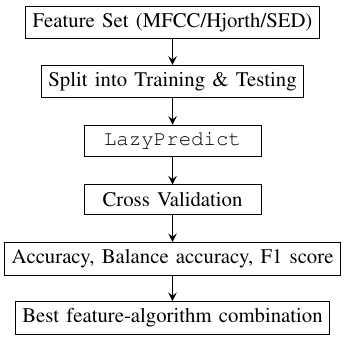
\includegraphics[width=5cm]{figures/algo}
	\caption{Determination of the best feature-algorithm combination for machine learning using {\tt lazy predict} platform. \textcolor{red}{Here, SED means spectral energy distribution.}}
	\label{fig_ML}
\end{figure}

\section{Experimental Data Collection}
The seismic signal collection was conducted at the elephant orphanage in Pinnawala, Sri Lanka (Figure \ref{fig:figure3nn}), where there are about twenty-five elephants in a free-ranging area.
\begin{figure}[t!]
	\centering   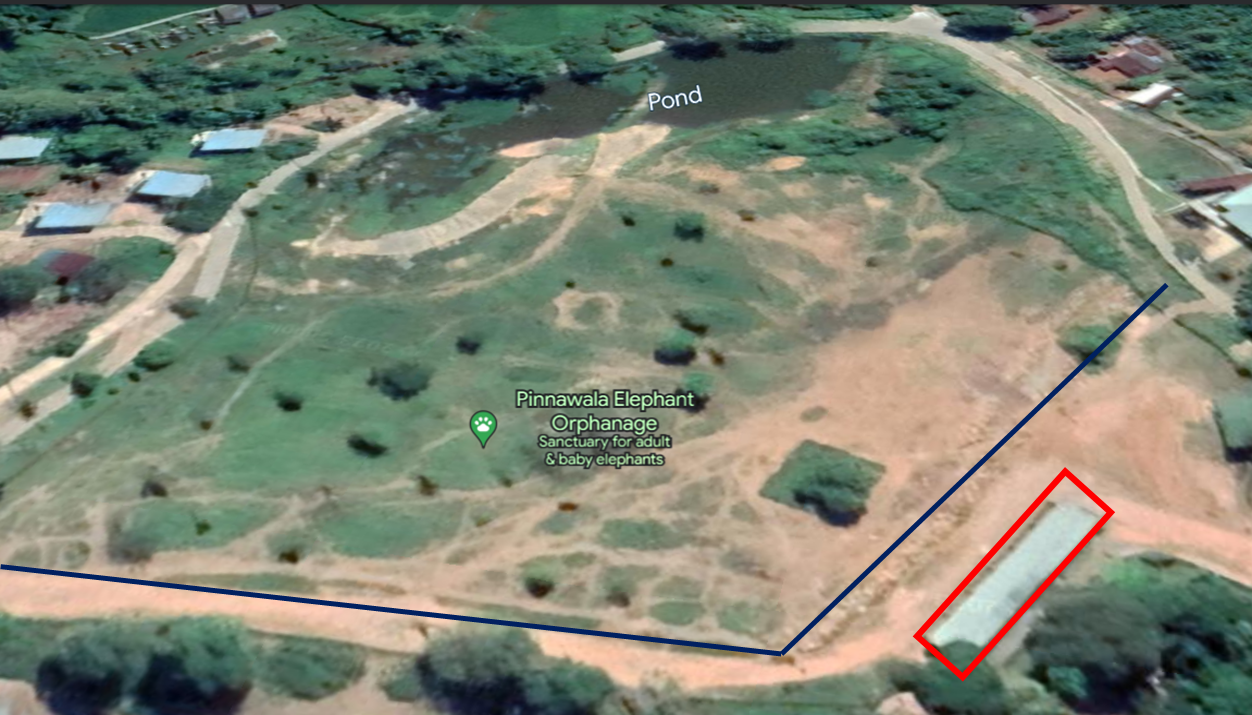
\includegraphics[width=4.5in]{figures/PinnawalaMap}
	\caption{Free ranging area in Pinnawala elephant orphanage. The observation hall is the marked rectangle closer to the right-bottom corner}
	\label{fig:figure3nn}
\end{figure}
The elephants’ behavior was closely observed before the experiment. It was clear that in hot weather, elephants tend to be inactive and spend most of the day under trees. However, in normal weather, they become active and engaged. Seismic data was collected under average weather conditions using three equispaced geophones buried near the fence that is marked with straight lines in Figure \ref{fig:figure3nn}. Elephant behavior was video recorded during the few-hour data capture. At the time the food truck arrived, one elephant rumbled quite noticeably as shown in Figure \ref{fig_rumble} where it shows that the elephant stands literally on two legs exerting maximum pressure on the ground that would enhance the seismic rumble propagate through the ground.
\begin{figure}
	\centering   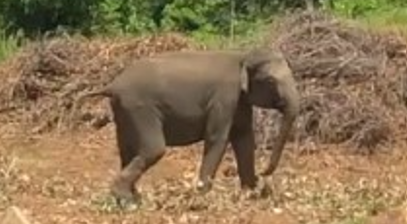
\includegraphics[width=4in]{figures/rumble.png}
	\caption{An elephant while rumbling - Pinnawala elephant orhpanage, Sri Lanka.}
	\label{fig_rumble}
\end{figure}
The seismic data that is aligned with audio and video records of the rumble was extracted from the recorded seismic signal. The spectrogram clearly shows the frequency patterns of strong elephant rumbles as shown at the 10 s mark of the top two illustrations of Figure \ref{fig_Spectograms}.
%\textcolor{red}{Our dataset contains 7 rumbles and 60 non-rumble instances.}
\begin{figure}[h]
	\centering
	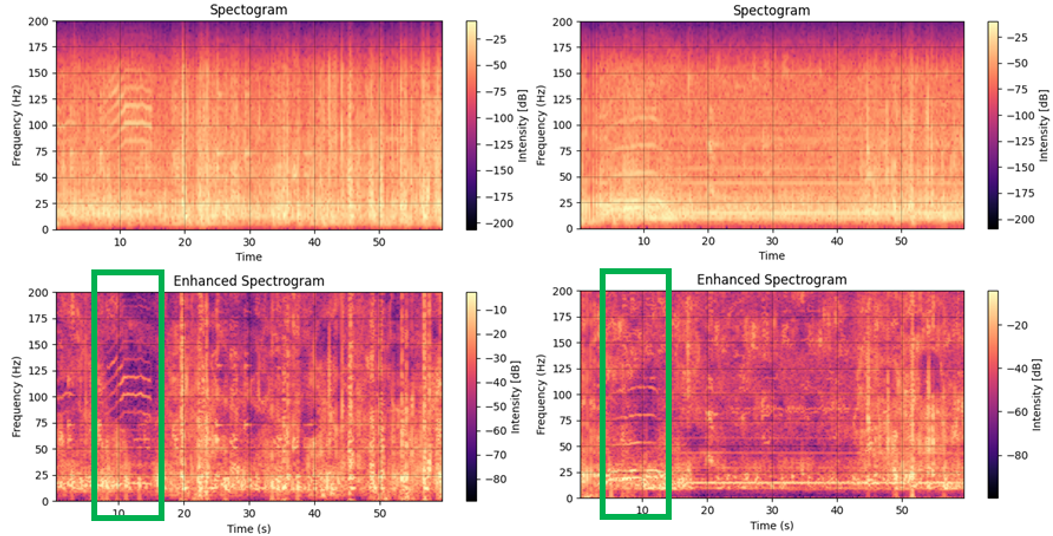
\includegraphics[width=5in]{figures/tworumbles.png}
	\caption{Spectrograms of two relatively strong rumbles verified by video-audio proof, before (top) and after (bottom) the enhancement using the proposed algorithm.}
	\label{fig_Spectograms}
\end{figure}
\section{Results}
The performance of each ML algorithm along with the relevant feature sets are compared using accuracy, balanced accuracy (BA) and F1 Score defines as follows:
\begin{eqnarray}
	Accuracy & =&  \frac{TP+TN}{TP+FP+TN+FN};\nonumber\\
	BA &=& \frac{Sensitivity+Specificity}{2};\nonumber\\
	F1~Score &=& \frac{2\times Precision\times Recall}{Precision + Recall};\nonumber
\end{eqnarray} in which
\begin{eqnarray}
	Sensitivity &=& \frac{TP}{TP+FN}\nonumber\\
	Specificity &=& \frac{TN}{TN+FP}\nonumber\\
	Precision &=&\frac{TP}{TP+FP}\nonumber\\
	Recall &=& \frac{TP}{TP+FN},\nonumber
\end{eqnarray}
where $TP$ is number of true positives, $FP$ is number of false positives, $TN$ is number of true negatives, and $FN$ is number of false negatives.

\subsection{Performance Comparison}

In this study, feature selection was based on p-values. Features with p-values below the threshold of 0.05 were considered significant to improve the model’s interpretability and reduce the risk of overfitting. Table \ref{MFCC_P_Value}, Table \ref{Hjorth_P_Value}, and Table \ref{Spectral_P_Value} show the selected features from MFCC features, Hjorth features, and Spectral energy features respectively. \\


\begin{table}[t!]
\centering
\begin{tabular}{|c|c|}
\hline
\textbf{MFCC Feature} & \textbf{P-Value} \\
\hline
mfcc\_2 & 4.198520e-11 \\
\hline
mfcc\_12 & 7.750290e-06 \\
\hline
mfcc\_22 & 3.081888e-04 \\
\hline
mfcc\_32 & 4.038959e-04 \\
\hline
mfcc\_7 & 6.701393e-04 \\
\hline
mfcc\_11 & 1.539645e-03 \\
\hline
mfcc\_30 & 1.756065e-03 \\
\hline
mfcc\_40 & 2.829550e-03 \\
\hline
mfcc\_21 & 2.907236e-03 \\
\hline
mfcc\_19 & 3.459980e-03 \\
\hline
mfcc\_29 & 1.106669e-02 \\
\hline
mfcc\_13 & 1.471919e-02 \\
\hline
mfcc\_9 & 1.511950e-02 \\
\hline
mfcc\_25 & 1.820666e-02 \\
\hline
mfcc\_38 & 3.290245e-02 \\
\hline
mfcc\_36 & 3.836483e-02 \\
\hline
mfcc\_31 & 4.856187e-02 \\
\hline
\end{tabular}
\caption{Selected MFCC features based on P values}
\label{MFCC_P_Value}
\end{table}



\begin{table}[t!]
\centering
\begin{tabular}{|c|c|}
\hline
\textbf{Feature} & \textbf{P-Value} \\
\hline
Activity & 0.001120 \\
\hline
Complexity & 0.043674 \\
\hline
Mobility & 0.044281 \\
\hline
\end{tabular}
\caption{Selected Hjorth features based on P values}
\label{Hjorth_P_Value}
\end{table}



\begin{table}[t!]
\centering
\begin{tabular}{|c|c|}
\hline
\textbf{Feature} & \textbf{P-Value} \\
\hline
SpecraEnergy\_14 & 0.007169 \\
\hline
SpecraEnergy\_15 & 0.009102 \\
\hline
SpecraEnergy\_13 & 0.038727 \\
\hline
SpecraEnergy\_16 & 0.039069 \\
\hline
\end{tabular}
\caption{Selected Spectral Energy features based on P values}
\label{Spectral_P_Value}
\end{table}

Table \ref{tab_MFCC} shows the rumble identification performance when the MFCC feature extraction method was used with the ridge classifier, SVM-linear, and Logistic regression as machine learning algorithms.

\begin{table}[h]
	\centering
	\begin{tabular}{|c|c|c|c|}
		\hline
		\textbf{ML Algorithm} & \textbf{Accuracy} & \textbf{BA} & \textbf{F1 score} \\
		\hline
		Ridge Classifier & 97.05 ± 0.051 \% & 95.83\% & 95.65\% \\
		\hline
		SVM-linear & 94.04 ± 0.067\% & 90\% & 88.89\% \\
		\hline
		Logistic Regression & 93.85  ± 0.069\% & 84.16\% & 77.78\% \\
		\hline
	\end{tabular}
	\caption{Performance when MFCCs were used as features}
	\label{tab_MFCC}
\end{table}

Table \ref{tab_Hj} shows the rumble identification performance when Hjorth parameters were used as features and the Decision tree classifier, AdaBoost classifier, and RandomForest classifier were used as machine learning algorithms. 
\begin{table}[h]
	\centering
	\begin{tabular}{|c|c|c|c|}
		\hline
		\textbf{ML Algorithm} & \textbf{Accuracy} & \textbf{BA} & \textbf{F1 score} \\
		\hline
		Decision Tree Classifier & 93.84 ± 0.096\% & 83.33\% & 73.68\% \\
		\hline
		AdaBoost Classifier & 92.26 ± 0.097\% & 78.33\% & 74.04\% \\
		\hline
		RandomForest Classifier & 89.68  ± 0.056\% & 70\% & 57.14\% \\
		\hline
	\end{tabular}
	\caption{Hjorth parameters as features}
	\label{tab_Hj}
\end{table}
Table \ref{tab_SED} shows the rumble identification performance when spectral energy distribution was used as features and LGBM classifier, Gradient boosting classifier, and AdaBoost classifier were used as machine learning algorithms. 
\begin{table}[H]
	\centering
	\begin{tabular}{|c|c|c|c|}
		\hline
		\textbf{ML Algorithm} & \textbf{Accuracy} & \textbf{BA} & \textbf{F1 score} \\
		\hline
		LGBM Classifier & 86.67 ± 0.119\% & 64.17\% & 42.86\% \\
		\hline
		Gradient Boosting Classifier & 81.95 ± 0.095\% & 63.33\% & 40\% \\
		\hline
		AdaBoost Classifier & 80.24  ± 0.136\% & 58.33\% & 28.57\% \\
		\hline
	\end{tabular}
	\caption{Spectral energy distribution as features}
	\label{tab_SED}
\end{table}
Based on the results in Table \ref{tab_MFCC} and Table\ref{tab_Hj}, MFCC with the Ridge classifier is the best combination for identifying elephant rumbles in seismic signals.

The performance of the best model for each feature extraction method was assessed using ROC curves, shown in Figures~\ref{fig:imgmfcc} to \ref{fig:imgspectr}. The Ridge Classifier performed exceptionally well with an AUC of 0.99, indicating near-perfect classification. The Decision Tree Classifier achieved an AUC of 0.88, while the LGBM Classifier reached a respectable 0.74. Overall, the combination of MFCC features and the Ridge Classifier is the most effective for the classification task.



\subsection{Effectiveness of Spectrogram Enhancement}
One of the main contributions of this work is spectrogram enhancement presented in \ref{subsub-SE}. It is evident qualitatively from Figure~\ref{fig_Spectograms} that the proposed approach enhance the features of the spectrogram. In order to compare the performance quantitatively, we employed the SSIM index. Here, we considered the spectrogram generated just after the ADC as the ground truth before any digital-domain processing and denoising. The achieved SSIM indices for the spectrograms enhanced using the proposed algorithm and that in~\cite{zeppelzauer2015towards} are presented in Table \ref{tab_denoise}. We note that higher SSIM means a more similarity for the original noisy spectrogram and vice versa. Accordingly, the low SSIM index achieved with the proposed algorithm indicate that proposed algorithm provides a better enhancement compared to the algorithm proposed in ~\cite{zeppelzauer2015towards}. 
\begin{table}[t!]
	\centering
	\begin{tabular}{|c|p{3cm}|p{3cm}|}
		\hline
		\textbf{Spectrogram} & \textbf{SSIM with the initial spectrum~\cite{zeppelzauer2015towards}} & \textbf{SSIM with the enhanced spectrum} \\
		\hline
		Fig.~\ref{fig_Spectograms}(left) & 0.86 &0.65\\
		\hline
		Fig.~\ref{fig_Spectograms}(right)& 0.89 & 0.66 \\
		\hline
	\end{tabular}
	\caption{Denoising effect in the spectrogram enhancement process, measured in SSIM index.}
	\label{tab_denoise}
\end{table}
%A low SSIM score indicates that fewer structural details are retained after spectrogram enhancement. The SSIM value drops by about 20\% with the spectrum enhancement.

\begin{figure}[H]
    \centering
    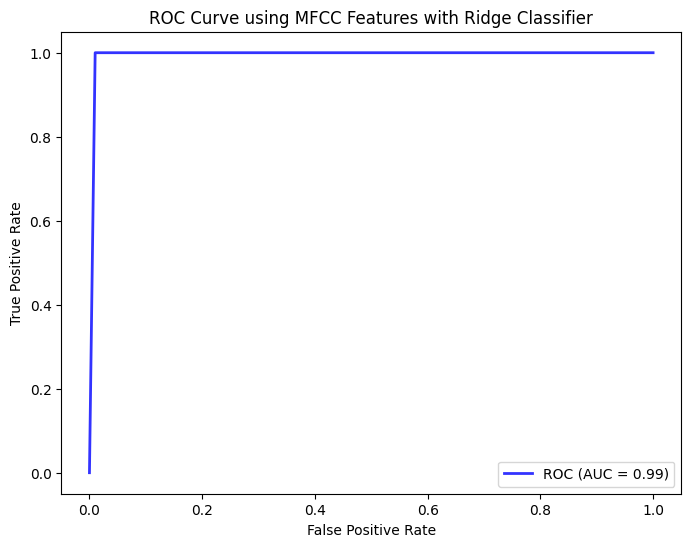
\includegraphics[width=3.5in]{figures/RidgeFull.png}
    \caption{ROC Curve using MFCC features with Ridge Classifier.}
    \label{fig:imgmfcc}
\vspace{0.3cm}
    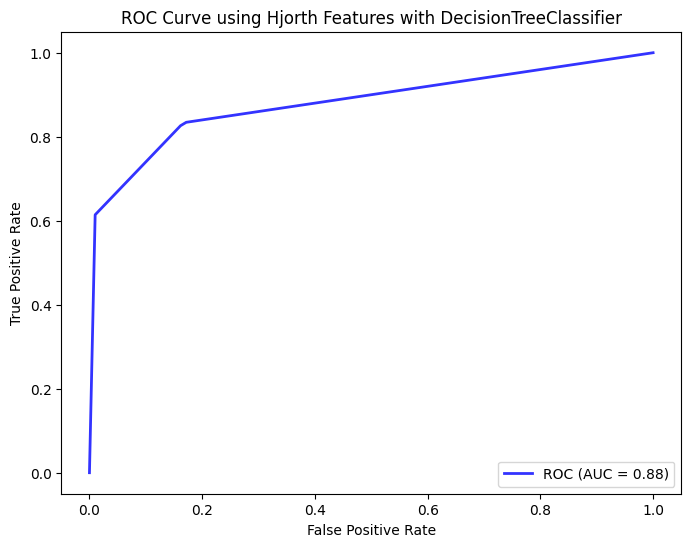
\includegraphics[width=3.5in]{figures/DesFull.png}
    \caption{ROC Curve using Hjorth features with Decision Tree Classifier.}
    \label{fig:imghjorth}
\vspace{0.3cm}
    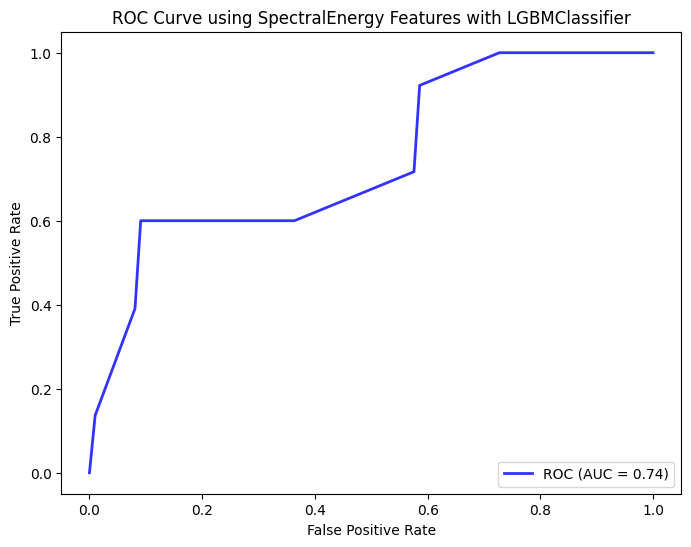
\includegraphics[width=3.5in]{figures/LGBMFull.png}
    \caption{ROC Curve using Spectral Energy features with LGBM Classifier.}
    \label{fig:imgspectr}
\end{figure}

\section{Conclusion}
The electronic circuitry and signal conditioning techniques have been developed quite successfully leading to acquiring seismic elephant rumbles in good quality. A few elephant rumbles were visually and audibly noticed during the data collection. Their seismic infrasonic copies were extracted from the geophone data, and the spectrograms were determined. The spectrogram enhancement has reduced noise in the seismic data quite significantly leading to achieving higher accuracy in feature detection and machine learning. Using {\tt lazy predict}, it was found that the MFCC feature extraction method and Ridge classifier ML algorithm give the best performance in automatic elephant rumble detection
.\par
The proposed elephant rumble identification method could be used to devise an early warning system for the villages troubled by wild elephants. The circuits involved are low-power and low-cost. It could be made even more cost-effective and less power-consuming by replacing the Raspberry Pi board with a Raspberry Pi zero board, which extends the battery life in field deployment. For the practical deployment, the best ML algorithm, Ridge classifier can be implemented on an edge device using {\tt scikit-learn} library in Python. It is important to mention that elephants do not rumble often, hence rumble detection will not lead to the development of a perfect early warning system. The elephant localization using seismic rumbles is yet to be investigated, though some early work has been reported.
%MDPI: Figure 9 is not cited in the main text, please confirm and add.
%MDPI: To avoid any changes to the figure, we have replaced it with a screenshot. Please confirm.
		

%MDPI: The following statements should be used ``Conceptualization, X.X. and Y.Y.; methodology, X.X.; software, X.X.; validation, X.X., Y.Y. and Z.Z.; formal analysis, X.X.; investigation, X.X.; resources, X.X.; data curation, X.X.; writing---original draft preparation, X.X.; writing---review and editing, X.X.; visualization, X.X.; supervision, X.X.; project administration, X.X.; funding acquisition, Y.Y. All authors have read and agreed to the published version of the manuscript.'', please turn to the  \href{http://img.mdpi.org/data/contributor-role-instruction.pdf}{CRediT taxonomy} for the term explanation. Authorship must be limited to those who have contributed substantially to the work~reported.
			
%\funding{This research received funding from National Research Council and AHEAD project. The Senate Research Committee of the University of Moratuwa provided the publication cost.}
%MDPI: Newly added, please confirm.
			
\institutionalreview{{Not applicable}}
%MDPI: In this section, please add the Institutional Review Board Statement and approval number for studies involving humans or animals. Please note that the Editorial Office might ask you for further information. Please add ``The study was conducted according to the guidelines of the Declaration of Helsinki, and approved by the Institutional Review Board (or Ethics Committee) of NAME OF INSTITUTE (protocol code XXX and date of approval).'' OR ``Ethical review and approval were waived for this study, due to REASON (please provide a detailed justification).'' OR ``Not applicable'' for studies not involving humans or animals. You might also choose to exclude this statement if the study did not involve humans or animals.
			
\informedconsent{{Not applicable}}
%MDPI: Any research article describing a study involving humans should contain this statement. Please add ``Informed consent was obtained from all subjects involved in the study.'' OR ``Patient consent was waived due to REASON (please provide a detailed justification).'' OR ``Not applicable'' for studies not involving humans. You might also choose to exclude this statement if the study did not involve humans. Written informed consent for publication must be obtained from participating patients who can be identified (including by the patients themselves). Please state ``Written informed consent has been obtained from the patient(s) to publish this paper'' if applicable.
			
\dataavailability{{Not available yet}} 
The video of the traditional and bird takeoff can be found at, https://www.youtube.com/watch?v=cu8rdGvTDYY
			
%MDPI: In this section, please provide details regarding where data supporting reported results can be found, including links to publicly archived datasets analyzed or generated during the study. Please refer to suggested Data Availability Statements in section ``MDPI Research Data Policies'' at \url{https://www.mdpi.com/ethics}. You might choose to exclude this statement if the study did not report any data.
			
\section*{Acknowledgment}
The authors would like to thank Dr. Daniela Hedwig, Director of the Elephant Listening Project, Dr. Geoffrey Abers, Chair of the Earth and Atmospheric Sciences at Cornell University, USA, and Dr. Chase A. LaDue, at Oklahoma City Zoo and Botanical Garden, USA for their insightful guidance.\par
Dr. Lori Lenard, Dr. Ronnie Coffman, and Dr. Richard Cahoon are acknowledged for facilitation and guidance provided for this research during the Fulbright Fellowship of the principal investigator Dr. Rohan Munasinghe at the Dept of Global Development, CALS, Cornell University, Ithaca, NY 14853, USA.\par
The authors would also acknowledge the staff of the National Zoological Department, and the Elephant Orphanage, Pinnawala, Sri Lanka for their approval and invaluable support during data collection.
			
\conflictsofinterest{{The authors declare no conflict of interest.}} 
%mdpi: Newly added, please confirm.
%\end{paracol}
\reftitle{References}
\begin{thebibliography}{999}
\bibitem{o2000seismic}
	O’Connell-Rodwell, C. E.; Arnason, B. T; and Hart, L. A.; \newblock Seismic properties of Asian elephant (Elephas maximus) vocalizations and locomotion.
	\newblock  The Journal of the Acoustical Society of America, vol. 108, no. 6, pp. 3066-3072, Acoustical Society of America, 2000.
	\bibitem{payne1986infrasonic}
	Payne, K. B; Langbauer, W. R; and Thomas, E. M; \newblock Infrasonic Calls of the Asian Elephant (Elephas Maximus).
	\newblock  The Journal of Behavioral Ecology and Sociobiology, vol. 18, no. 4, pp. 297-301, Springer, 1986.
\bibitem{sayakkara2017eloc}
	Sayakkara, A. P.; Jayasuriya, N.; Ranathunga, T.; Suduwella, C.; Vithanage, N.; Keppitiyagama, C.; De Zoysa, K.; Hewage, K.; and Voigt, T.; \newblock Eloc: locating wild elephants using low-cost infrasonic detectors.
	\newblock 13th IEEE International Conference on Distributed Computing in Sensor Systems (DCOSS), pp. 44-52, 2017.
\bibitem{zeppelzauer2015towards}
	Zeppelzauer, M.; Hensman, S.; and Stoeger, A. S.; \newblock Towards an automated acoustic detection system for free-ranging elephants.
	\newblock Bioacoustics, vol. 24, no. 1, pp. 13-29, Taylor \& Francis, 2015.
\bibitem{Reinwald2021}
	Reinwald, M.; Moseley, B.; Szenicer, A.; Nissen-Meyer, T.; Oduor, S.; Vollrath1, F.; Markham A.; and Mortimer, B.; \newblock Seismic localization of elephant rumbles as a monitoring approach.
	\newblock Interface, vol. 18, pp. 1-11, The Royal Society, 2021.
\bibitem{nair2009vocalizations}
	Nair, S.; Balakrishnan, R.; Seelamantula, C. S.; and Sukumar, R.; \newblock Vocalizations of wild Asian elephants (Elephas maximus): structural classification and social context.
	\newblock The Journal of the Acoustical Society of America, vol. 126, no. 5, pp. 2768-2778, 2009.
\bibitem{phinyomark2012usefulness}
	Phinyomark, A.; Phukpattaranont, P.; and Limsakul, C.; \newblock The usefulness of wavelet transform to reduce noise in the SEMG signal.
	\newblock EMG methods for evaluating muscle and nerve function, pp. 107-132, nTech Rijeka, Croatia, 2012.
\bibitem{Daubechies}
	Daubechies, I.; \newblock Orthonormal bases of compactly supported wavelets.
	\newblock Communications on Pure and Applied Mathematics, vol. 41, no. 7, pp. 909-996, Wiley, 1988.
\bibitem{wannawijit2019ecg}
	Wannawijit, I.; and Kaiwansil, S.; Ruthaisujaritkul, S.; and Yingthawornsuk, T.; \newblock ECG classification with modification of higher-order Hjorth descriptors.
	\newblock In Proc. 2019 15th IEEE International Conference on Signal-Image Technology \& Internet-Based Systems (SITIS), pp. 564-571, 2019.
\bibitem{wang2004image}
	Wang, Z.; Bovik, A. C.; Sheikh, H. R.; and Simoncelli, E. P.; \newblock Image quality assessment: from error visibility to structural similarity.
	\newblock IEEE transactions on image processing, vol. 13, no. 4, pp. 600-612, 2004.
\bibitem{clemins2006generalized}
	Clemins, P. J.; Johnson, M. T.; \newblock Generalized perceptual linear prediction features for animal vocalization analysis.
	\newblock The Journal of the Acoustical Society of America, vol. 120, no. 1, pp. 527-534, AIP Publishing, 2006.
\bibitem{kim2011sound}
	Kim, Y-E.; Su, D-H.; Jeon, C-H.; Lee, J-K.; Cho, K-J.; Chung, J-G.; \newblock Sound Source Localization Method Using Region Selection.
	\newblock Advances in Sound Localization, IntecOpen, 2011.
\bibitem{gunther2004seismic}
	G{\"u}nther, R. H.; O'Connell-Rodwell, C. E.; Caitlin, E.; and Klemperer. S. L.; \newblock Seismic waves from elephant vocalizations: A possible communication mode?.
	\newblock Geophysical Research Letters, vol. 31, no. 11, Wiley Online Library, 2004.
\bibitem{oppenheim1999discrete}
	Oppenheim, A. V.; \newblock Discrete-time signal processing. Ed.3
	\newblock Pearson Higher Education Inc., Upper Saddle River, NJ, 2010.
\bibitem{jurafsky}
	Jurafsky, D.; and Martin, J. H.; \newblock Speech and Language Processing, Ed. 3
	\newblock Online available, 2003.
\bibitem{keen2017automated}
	Keen, S. C.; Shiu, Y.; Wrege, P. H.; and Rowland, E. D.; \newblock Automated detection of low-frequency rumbles of forest elephants: A critical tool for their conservation
	\newblock The Journal of the Acoustical Society of America, vol. 141, no. 4, pp. 2715-2726, AIP Publishing, 2017.
\bibitem{zumbahlen2007phase}
	Zumbahlen, H.; \newblock Phase Relations in Active Filters
	\newblock Analog Dialogue, vol. 41, no. 4, 2007.
\bibitem{linghu2022ensemble}
	Linghu, J.; and Dong, H.; and Cui, J.; \newblock Ensemble wavelet-learning approach for predicting the effective mechanical properties of concrete composite materials
	\newblock Computational Mechanics, vol. 70, no. 2, pp. 335--365, 2022.
\bibitem{scikit-learn}
	Pedregosa, F.; Varoquaux, G.; Gramfort, A.; Michel, V.; Thirion, B.; Grisel, O.; Blondel, M.; Prettenhofer, P.; Weiss, R.; Dubourg, V.; Vanderplas, J.; Passos, A.; Cournapeau, D.; Brucher, M.; Perrot, M.; and Duchesnay, E.; \newblock Ensemble wavelet-learning approach for predicting the effective mechanical properties of concrete composite materials
	\newblock Journal of Machine Learning Research, vol. 12, pp. 2825--2830, 2011.
\bibitem{donoho1995noising}
	Donoho, D. L.; \newblock De-noising by soft-thresholding
	\newblock IEEE transactions on information theory, vol. 41, no. 3, pp. 613-627, 1995.
\bibitem{prakash}
	Prakash, T, G,; Supun L.; Wijeratne, A. W.; and Fernando, P.; \newblock Human-Elephant Conflict in Sri Lanka: Patterns and Extent
	\newblock Gajah, vol. 51, pp. 16-25, IUCN/SSC Asian Elephant Specialist Group, 2020.
\bibitem{wijayakulasooriya}
	Wijayakulasooriya, J. V.; \newblock Automatic recognition of elephant infrasound calls using formant analysis and hidden markov model
	\newblock Proceedings of the international conference on industrial and information
	systems, pp. 244-248, 2011.
\bibitem{zeppelzauer2015}
	Zeppelzauer, M.; Stoeger, A. S.; and Breiteneder, C.; \newblock Acoustic Detection of Elephant Presence in Noisy Environments
	\newblock Proceedings of the 2nd ACM International Workshop on Multimedia Analysis for Ecological Data, pp. 3-8, ACM Press,2013.
\bibitem{Hao}
	Hao, Y.; Campana, B.; and Keogh, E.; \newblock Monitoring and mining animal sounds in visual space
	\newblock ournal of Insect Behavior, vol. 26, no. 4, pp. 466-493, 2012.
\end{thebibliography}
\end{document}